% !TeX program = xelatex
\documentclass[a4paper,10pt]{article}

% ============================================================================
% ១. កញ្ចប់បណ្ណាល័យ និងការកំណត់ទំព័រ (Packages & Page Setup — តាមគំរូ ls_plan.tex)
% ============================================================================
\usepackage[a4paper, left=0.95cm, right=0.95cm, top=0.85cm, bottom=0.92cm, footskip=0.52cm]{geometry}
\usepackage{amsmath}
\usepackage{unicode-math}
\usepackage{fontspec}
\usepackage{longtable, array, multirow, colortbl}
\usepackage[table]{xcolor}
\usepackage{enumitem}
\usepackage{pifont}
\usepackage{fancyhdr}
\usepackage{tikz}
\usetikzlibrary{calc, arrows.meta, decorations.pathreplacing, patterns, positioning, babel}

\makeatletter
\let\@expl@@@mark@update@singlecol@structures@@\relax
\makeatother

% --- ប្រព័ន្ធស្វែងរកទីតាំងពុម្ពអក្សរស្វ័យប្រវត្តិ (Windows Local + Cloud Repo fonts/) ---
\providecommand{\NGSFindFonts}{%
  \IfFileExists{C:/Windows/Fonts/cambria.ttc}{%
    \def\NGSSysPath{C:/Windows/Fonts/}%
    \def\NGSUserPath{C:/Users/KIT/AppData/Local/Microsoft/Windows/Fonts/}%
  }{%
    \IfFileExists{./fonts/KhmerOSsiemreap.ttf}{\def\NGSSysPath{./fonts/}\def\NGSUserPath{./fonts/}}{%
    \IfFileExists{../fonts/KhmerOSsiemreap.ttf}{\def\NGSSysPath{../fonts/}\def\NGSUserPath{../fonts/}}{%
    \IfFileExists{../../fonts/KhmerOSsiemreap.ttf}{\def\NGSSysPath{../../fonts/}\def\NGSUserPath{../../fonts/}}{%
    \IfFileExists{../../../fonts/KhmerOSsiemreap.ttf}{\def\NGSSysPath{../../../fonts/}\def\NGSUserPath{../../../fonts/}}{%
    \IfFileExists{../../../../fonts/KhmerOSsiemreap.ttf}{\def\NGSSysPath{../../../../fonts/}\def\NGSUserPath{../../../../fonts/}}{%
    \IfFileExists{../../../../../fonts/KhmerOSsiemreap.ttf}{\def\NGSSysPath{../../../../../fonts/}\def\NGSUserPath{../../../../../fonts/}}{%
    \IfFileExists{../../../../../../fonts/KhmerOSsiemreap.ttf}{\def\NGSSysPath{../../../../../../fonts/}\def\NGSUserPath{../../../../../../fonts/}}{%
      \def\NGSSysPath{../../../../../../../fonts/}\def\NGSUserPath{../../../../../../../fonts/}%
    }}}}}}}%
  }%
}
\NGSFindFonts

% ============================================================================
% ២. កំណត់ពុម្ពអក្សរ (Fonts — តាមគំរូ ls_plan.tex)
% ============================================================================
\setmathfont[Path={\NGSSysPath}, FontIndex=1, Scale=1.02]{cambria.ttc}
\defaultfontfeatures{Ligatures=TeX}

\setmainfont[
  Path={\NGSUserPath},
  Extension=.ttf,
  Script=Khmer,
  BoldFont={KhmerOSsiemreap},
  BoldFeatures={FakeBold=1.8},
  ItalicFont={KhmerOSsiemreap},
  ItalicFeatures={FakeSlant=0.25},
  BoldItalicFont={KhmerOSsiemreap},
  BoldItalicFeatures={FakeBold=1.8, FakeSlant=0.25}
]{KhmerOSsiemreap}

\newfontfamily\muol[Path={\NGSUserPath}, Extension=.ttf, Script=Khmer]{KhmerOSmuollight}
\newfontfamily\Tacteing[Path={\NGSUserPath}, Extension=.TTF]{TACTENG}
\newfontfamily\TimesEn[Path={\NGSSysPath}, Extension=.ttf, BoldFont={timesbd}, ItalicFont={timesi}, BoldItalicFont={timesbi}]{times}
\newfontfamily\CalibriFont[Path={\NGSSysPath}, Extension=.ttf]{calibri}
\newfontfamily\CourierCirc[Path={\NGSSysPath}, Extension=.ttf]{cour}

\XeTeXlinebreaklocale "km"
\XeTeXlinebreakskip = 0pt plus 1pt minus 0.1pt

% ============================================================================
% ៣. ពណ៌ និងការតុបតែង (Colors & Styles)
% ============================================================================
\definecolor{stepbg}{HTML}{D9D9D9}
\definecolor{headgray}{HTML}{E6E6E6}
\definecolor{emphred}{HTML}{C00000}

\pagestyle{fancy}
\fancyhf{}
\renewcommand{\headrulewidth}{0pt}
\fancyfoot[R]{\CalibriFont\fontsize{9pt}{11pt}\selectfont\thepage}

\setlength{\parindent}{0pt}
\setlength{\parskip}{0pt}
\setlength{\tabcolsep}{4.5pt}
\setlength{\LTpre}{2pt}
\setlength{\LTpost}{2pt}

\newcolumntype{L}[1]{>{\raggedright\arraybackslash}p{#1}}
\newcolumntype{C}[1]{>{\centering\arraybackslash}p{#1}}

% ============================================================================
% ៤. ពាក្យបញ្ជាជំនួយ (Helper Macros)
% ============================================================================
\newcommand{\en}[1]{{\TimesEn #1}}
\newcommand{\enbf}[1]{{\TimesEn\bfseries #1}}
\newcommand{\khmflourish}{{\Tacteing\fontsize{15pt}{15pt}\selectfont 3}}
\newcommand{\wcirc}{{\CourierCirc\fontsize{9.5pt}{11pt}\selectfont o}}
\newcommand{\ditem}{{\fontsize{7.5pt}{10pt}\selectfont\ding{117}}\ }
\newcommand{\fiveE}[1]{\textcolor{emphred}{\CalibriFont\bfseries #1}}
\newcommand{\redsub}[1]{\textcolor{emphred}{#1}}
\newcommand{\timenote}[1]{\textcolor{emphred}{\textit{#1}}}
\newcommand{\stepheader}[1]{\multicolumn{3}{|c|}{\cellcolor{stepbg}\muol #1} \\ \hline}
\newcommand{\cfig}[1]{{\centering\vspace{3pt}#1\vspace{3pt}\par}}
\newcommand{\cnum}[1]{\mbox{\fontsize{10.5pt}{12pt}\selectfont\ding{\numexpr181+#1\relax}}}
\newcommand{\unit}[1]{\,\text{\en{#1}}}
\newcommand{\graybox}[1]{\colorbox{headgray}{\strut #1}}

% ============================================================================
% ៥. រូបភាព TikZ ស-ខ្មៅ សម្រាប់បង្រៀនលើក្ដារខៀន និងសន្លឹកកិច្ចការ (B&W Diagrams)
% ============================================================================

% ១. E1 Engage: អន្ទាក់ភ្លេចរំកិលខ្ទង់ក្នុងផលគុណរង 7428 x 64 (ទំ.៥)
\newcommand{\figEngageWNOneThree}{%
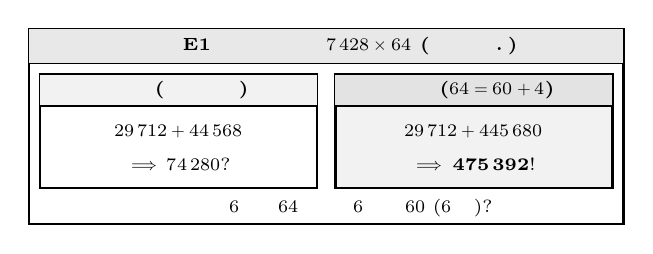
\begin{tikzpicture}[x=1cm, y=1cm, every node/.style={font=\fontsize{6.4pt}{8.4pt}\selectfont, text=black}]
  \draw[black, line width=0.9pt] (0,0) rectangle (7.55,2.48);
  \fill[gray!18] (0,2.04) rectangle (7.55,2.48);
  \draw[black, line width=0.6pt] (0,2.04) -- (7.55,2.04);
  \node at (3.775,2.26) {\textbf{បេសកកម្ម \en{E1}៖ អន្ទាក់ផលគុណរងក្នុង $7\,428 \times 64$ (ឧទាហរណ៍ ២ ទំ.៥)}};

  % Left: Student A
  \draw[black, line width=0.8pt] (0.14,0.46) rectangle (3.66,1.90);
  \fill[gray!10] (0.14,1.50) rectangle (3.66,1.90);
  \draw[black, line width=0.5pt] (0.14,1.50) -- (3.66,1.50);
  \node at (1.90,1.70) {\textbf{សិស្ស ក (ភ្លេចរំកិលខ្ទង់)}};
  \node at (1.90,1.18) {$29\,712 + 44\,568$};
  \node at (1.90,0.76) {$\implies 74\,280$?};

  % Right: Student B
  \draw[black, line width=0.95pt, fill=gray!10] (3.89,0.46) rectangle (7.41,1.90);
  \fill[gray!22] (3.89,1.50) rectangle (7.41,1.90);
  \draw[black, line width=0.55pt] (3.89,1.50) -- (7.41,1.50);
  \node at (5.65,1.70) {\textbf{សិស្ស ខ ($64 = 60 + 4$)}};
  \node at (5.65,1.18) {$29\,712 + 445\,680$};
  \node at (5.65,0.76) {$\implies \mathbf{475\,392}$!};

  \node at (3.775,0.21) {\textbf{សំណួរ៖} តើលេខ $6$ ក្នុង $64$ តំណាងឱ្យ $6$ រាយ ឬ $60$ ($6$ ដប់)?};
\end{tikzpicture}}

% ២. E2 Explore: ផលគុណរង 7428 x 64 និងវិធីចែកអឺគ្លីត 5406 : 128 (ទំ.៥)
\newcommand{\figMultDivWNOneThree}{%
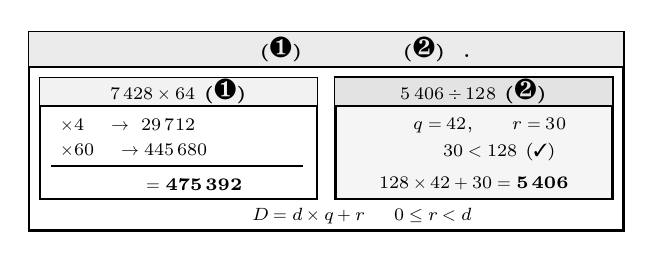
\begin{tikzpicture}[x=1cm, y=1cm, every node/.style={font=\fontsize{6.4pt}{8.4pt}\selectfont, text=black}]
  \draw[black, line width=0.9pt] (0,0) rectangle (7.55,2.52);
  \fill[gray!16] (0,2.08) rectangle (7.55,2.52);
  \draw[black, line width=0.6pt] (0,2.08) -- (7.55,2.08);
  \node at (3.775,2.30) {\textbf{ផលគុណរងតាមខ្ទង់ (\cnum{1}) និងវិធីចែកអឺគ្លីត (\cnum{2}) ទំ.៥}};

  % Left: Multiplication 7428 x 64
  \draw[black, line width=0.8pt] (0.14,0.40) rectangle (3.66,1.94);
  \fill[gray!10] (0.14,1.58) rectangle (3.66,1.94);
  \draw[black, line width=0.5pt] (0.14,1.58) -- (3.66,1.58);
  \node at (1.90,1.76) {\textbf{$7\,428 \times 64$ (\cnum{1})}};
  \node[anchor=west] at (0.28,1.34) {$\times 4\text{ រាយ} \to \ 29\,712$};
  \node[anchor=west] at (0.28,1.02) {$\times 60\text{ ដប់} \to 445\,680$};
  \draw[black, line width=0.6pt] (0.28,0.82) -- (3.48,0.82);
  \node at (1.90,0.58) {ផលគុណ $=\mathbf{475\,392}$};

  % Right: Division 5406 : 128
  \draw[black, line width=0.95pt, fill=gray!8] (3.89,0.40) rectangle (7.41,1.94);
  \fill[gray!22] (3.89,1.58) rectangle (7.41,1.94);
  \draw[black, line width=0.55pt] (3.89,1.58) -- (7.41,1.58);
  \node at (5.65,1.76) {\textbf{$5\,406 \div 128$ (\cnum{2})}};
  \node at (5.65,1.34) {ផលចែក $q = 42$, សំណល់ $r = 30$};
  \node at (5.65,1.00) {លក្ខខណ្ឌ៖ $30 < 128$ (\ding{51})};
  \node at (5.65,0.60) {$128 \times 42 + 30 = \mathbf{5\,406}$};

  \node at (3.775,0.18) {សមភាពអឺគ្លីត៖ $D = d \times q + r$ ដែល $0 \le r < d$};
\end{tikzpicture}}

% ៣. E3 Explain: ទំនាក់ទំនងច្រាសរវាងវិធីគុណនិងវិធីចែក (ទំ.៦)
\newcommand{\figInverseWNOneThree}{%
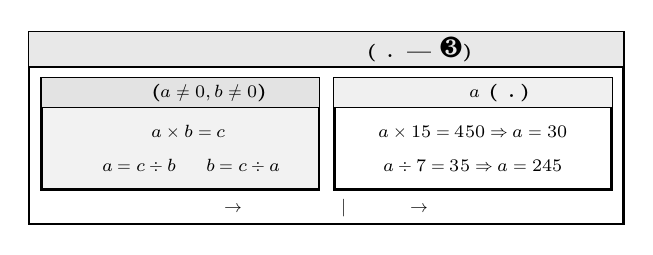
\begin{tikzpicture}[x=1cm, y=1cm, every node/.style={font=\fontsize{6.4pt}{8.4pt}\selectfont, text=black}]
  \draw[black, line width=0.9pt] (0,0) rectangle (7.55,2.44);
  \fill[gray!18] (0,2.00) rectangle (7.55,2.44);
  \draw[black, line width=0.6pt] (0,2.00) -- (7.55,2.00);
  \node at (3.775,2.22) {\textbf{ទំនាក់ទំនងច្រាសរវាងវិធីគុណនិងវិធីចែក (ទំ.៦ — \cnum{3})}};

  % Left box: Exact division inverse
  \draw[black, line width=0.85pt, fill=gray!10] (0.16,0.44) rectangle (3.68,1.86);
  \fill[gray!22] (0.16,1.48) rectangle (3.68,1.86);
  \draw[black, line width=0.5pt] (0.16,1.48) -- (3.68,1.48);
  \node at (1.92,1.67) {\textbf{វិធានច្រាស ($a\ne 0, b\ne 0$)}};
  \node at (1.92,1.18) {បើ $a \times b = c$};
  \node at (1.92,0.74) {នោះ $a = c \div b$ និង $b = c \div a$};

  % Right box: Examples from p.6
  \draw[black, line width=0.85pt] (3.88,0.44) rectangle (7.40,1.86);
  \fill[gray!12] (3.88,1.48) rectangle (7.40,1.86);
  \draw[black, line width=0.5pt] (3.88,1.48) -- (7.40,1.48);
  \node at (5.64,1.67) {\textbf{ឧទាហរណ៍រក $a$ (ទំ.៦)}};
  \node at (5.64,1.18) {$a \times 15 = 450 \Rightarrow a = 30$};
  \node at (5.64,0.74) {$a \div 7 = 35 \Rightarrow a = 245$};

  \node at (3.775,0.20) {រកកត្តាមិនស្គាល់ $\to$ ចែកនឹងកត្តាស្គាល់ $\mid$ រកតំណាងចែក $\to$ គុណតួចែកនឹងផលចែក};
\end{tikzpicture}}

% ៤. E4 Elaborate: លំហាត់គំរូ ១ និង ២ (ទំ.៦ — បណ្ណាគារ និងតុសិស្ស)
\newcommand{\figModelsWNOneThree}{%
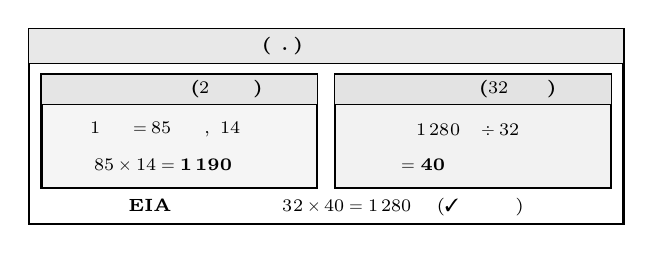
\begin{tikzpicture}[x=1cm, y=1cm, every node/.style={font=\fontsize{6.4pt}{8.4pt}\selectfont, text=black}]
  \draw[black, line width=0.9pt] (0,0) rectangle (7.55,2.48);
  \fill[gray!18] (0,2.04) rectangle (7.55,2.48);
  \draw[black, line width=0.6pt] (0,2.04) -- (7.55,2.04);
  \node at (3.775,2.26) {\textbf{លំហាត់គំរូ ១ និង ២ (ទំ.៦)៖ ចំណោទវិធីគុណ និងវិធីចែកចំណែកស្មើគ្នា}};

  % Model 1: Bookstore
  \draw[black, line width=0.8pt, fill=gray!8] (0.16,0.46) rectangle (3.66,1.90);
  \fill[gray!20] (0.16,1.52) rectangle (3.66,1.90);
  \draw[black, line width=0.5pt] (0.16,1.52) -- (3.66,1.52);
  \node at (1.91,1.71) {\textbf{គំរូ ១៖ បណ្ណាគារ ($2$ សប្ដាហ៍)}};
  \node at (1.91,1.20) {$1\text{ ថ្ងៃ} = 85\text{ ក្បាល}, \ 14\text{ ថ្ងៃ}$};
  \node at (1.91,0.76) {$85 \times 14 = \mathbf{1\,190\text{ \textbf{ក្បាល}}}$};

  % Model 2: School desks
  \draw[black, line width=0.85pt, fill=gray!10] (3.89,0.46) rectangle (7.39,1.90);
  \fill[gray!22] (3.89,1.52) rectangle (7.39,1.90);
  \draw[black, line width=0.5pt] (3.89,1.52) -- (7.39,1.52);
  \node at (5.64,1.71) {\textbf{គំរូ ២៖ តុសិស្ស ($32$ បន្ទប់)}};
  \node at (5.64,1.20) {សរុប $1\,280\text{ តុ} \div 32\text{ បន្ទប់}$};
  \node at (5.64,0.76) {$= \mathbf{40\text{ \textbf{តុ}}}$ ក្នុង ១ បន្ទប់};

  \node at (3.775,0.22) {\textbf{\en{EIA}៖} ផ្ទៀងផ្ទាត់គំរូ ២៖ $32 \times 40 = 1\,280$ តុ (\ding{51} ត្រឹមត្រូវ)};
\end{tikzpicture}}

% ៥. E5 Evaluate: ជម្រើសវិនិច្ឆ័យ A-D លើវិធីចែកមានសំណល់ និងផលគុណរង
\newcommand{\figExitWNOneThree}{%
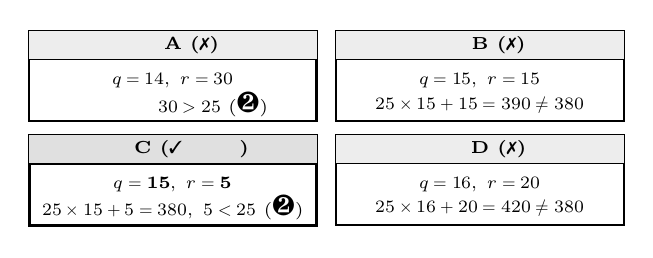
\begin{tikzpicture}[x=1cm, y=1cm, every node/.style={font=\fontsize{6.3pt}{8.2pt}\selectfont, text=black}]
  % Choice A
  \draw[black, line width=0.8pt] (0,1.32) rectangle (3.65,2.46);
  \fill[gray!14] (0,2.10) rectangle (3.65,2.46);
  \draw[black, line width=0.5pt] (0,2.10) -- (3.65,2.10);
  \node at (1.825,2.28) {\textbf{ជម្រើស \en{A} (\ding{55})}};
  \node at (1.825,1.84) {$q = 14, \ r = 30$};
  \node at (1.825,1.53) {សំណល់ធំជាងតួចែក $30 > 25$ (\cnum{2})};

  % Choice B
  \draw[black, line width=0.8pt] (3.90,1.32) rectangle (7.55,2.46);
  \fill[gray!14] (3.90,2.10) rectangle (7.55,2.46);
  \draw[black, line width=0.5pt] (3.90,2.10) -- (7.55,2.10);
  \node at (5.725,2.28) {\textbf{ជម្រើស \en{B} (\ding{55})}};
  \node at (5.725,1.84) {$q = 15, \ r = 15$};
  \node at (5.725,1.53) {$25\times 15 + 15 = 390 \ne 380$};

  % Choice C (Correct)
  \draw[black, line width=1.05pt] (0,0) rectangle (3.65,1.14);
  \fill[gray!24] (0,0.78) rectangle (3.65,1.14);
  \draw[black, line width=0.6pt] (0,0.78) -- (3.65,0.78);
  \node at (1.825,0.96) {\textbf{ជម្រើស \en{C} (\ding{51} ត្រឹមត្រូវ)}};
  \node at (1.825,0.52) {$q = \mathbf{15}, \ r = \mathbf{5}$};
  \node at (1.825,0.22) {$25\times 15 + 5 = 380,\ 5<25$ (\cnum{2})};

  % Choice D
  \draw[black, line width=0.8pt] (3.90,0) rectangle (7.55,1.14);
  \fill[gray!14] (3.90,0.78) rectangle (7.55,1.14);
  \draw[black, line width=0.5pt] (3.90,0.78) -- (7.55,0.78);
  \node at (5.725,0.96) {\textbf{ជម្រើស \en{D} (\ding{55})}};
  \node at (5.725,0.52) {$q = 16, \ r = 20$};
  \node at (5.725,0.22) {$25\times 16 + 20 = 420 \ne 380$};
\end{tikzpicture}}

\begin{document}
\fontsize{10pt}{15.2pt}\selectfont

% ============================================================================
% ក្បាលរដ្ឋបាល (Administrative Header — តាមគំរូ ls_plan.tex)
% ============================================================================
{\centering
  {\muol\fontsize{11pt}{16pt}\selectfont ព្រះរាជាណាចក្រកម្ពុជា\par}
  {\muol\fontsize{11pt}{16pt}\selectfont ជាតិ សាសនា ព្រះមហាក្សត្រ\par}
  \vspace{-3pt}{\khmflourish\par}
}

\vspace{1pt}
{\muol\fontsize{10pt}{15.5pt}\selectfont
មន្ទីរអប់រំ យុវជន និងកីឡា ខេត្តកំពង់ធំ\par
ការិយាល័យអប់រំ យុវជន និងកីឡា ស្រុកកំពង់ស្វាយ\par
អនុវិទ្យាល័យព្រះក្រសាំង\par}

\vspace{2pt}
{\centering{\muol\fontsize{11.5pt}{17pt}\selectfont កិច្ចតែងការបង្រៀន\par}}
\vspace{2pt}

% --- ព័ត៌មានទូទៅ ---
{\hspace*{2.8cm}\renewcommand{\arraystretch}{1.08}
\begin{tabular}{@{}l@{\hspace{0.35cm}}p{2.9cm}@{\hspace{0.15cm}}c@{\hspace{0.25cm}}l@{}}
  - & មុខវិជ្ជា & : & គណិតវិទ្យា ថ្នាក់ទី៧ (ពីជគណិត) \\
  - & ចំណងជើងមេរៀន & : & មេរៀនទី១៖ ចំនួនគត់ \\
  - & ចំណងជើងរង & : & ៤.២ វិធីគុណនិងវិធីចែកចំនួនគត់ (ទំ.៤--៦) \\
  - & រយៈពេល & : & ១ ម៉ោងសិក្សា (៥០ នាទី) \\
  - & បង្រៀនដោយ & : & ហុក ប៊ុនថែន \\
  - & កាលបរិច្ឆេទ & : & ថ្ងៃព្រហស្បតិ៍ ទី៥ ខែវិច្ឆិកា ឆ្នាំ២០២៦ \\
\end{tabular}\par}

\vspace{2pt}

% --- I. វត្ថុបំណង ---
{\muol\fontsize{10pt}{15.5pt}\selectfont \enbf{I.} វត្ថុបំណង\par}
\vspace{1pt}
{\renewcommand{\arraystretch}{1.10}
\begin{tabular}{@{}p{0.55cm}@{}p{2.35cm}@{\hspace{0.15cm}}c@{\hspace{0.25cm}}p{14.95cm}@{}}
  \hfill\wcirc\hspace{0.2cm} & វិជ្ជាសម្បទា & : & សិស្សប្រាប់បានពីអត្ថន័យនៃផលគុណរងតាមតម្លៃខ្ទង់ សមភាពនៃវិធីចែកអឺគ្លីត ($D = d\times q + r, \ 0 \le r < d$) និងទំនាក់ទំនងច្រាសរវាងវិធីគុណនិងវិធីចែក ($a\times b = c \iff a=c\div b, b=c\div a$) បានត្រឹមត្រូវ ។ \\
  \hfill\wcirc\hspace{0.2cm} & បំណិនសម្បទា & : & សិស្សគណនាផលគុណនិងផលចែកចំនួនគត់ច្រើនខ្ទង់ រកតួមិនស្គាល់ និងដោះស្រាយចំណោទជីវភាពពិត (ការលក់សៀវភៅក្នុងបណ្ណាគារ និងការបែងចែកតុសិស្ស ទំ.៦) លើសន្លឹកកិច្ចការបានត្រឹមត្រូវ ។ \\
  \hfill\wcirc\hspace{0.2cm} & ចរិយាសម្បទា & : & សិស្សមានទម្លាប់ផ្ទៀងផ្ទាត់ផលចែកនិងសំណល់តាមសមភាព $D = d\times q + r$ មានភាពហ្មត់ចត់ក្នុងការរំកិលខ្ទង់ផលគុណរង និងសហការគ្នាដោះស្រាយបញ្ហាជាក្រុម ។ \\
\end{tabular}\par}

\vspace{2pt}

% --- II. សម្ភារៈឧបទេស ---
{\muol\fontsize{10pt}{15.5pt}\selectfont \enbf{II.} សម្ភារៈឧបទេស\par}
\vspace{1pt}
\hspace*{0.55cm}$\bullet$\ សៀវភៅសិក្សាគោលថ្នាក់ទី៧ (ទំ.៤--៦ និងទំ.១៤) ក្ដារខៀន ដីស/ហ្វឺត បន្ទាត់ត្រង់ និង\textbf{សន្លឹកកិច្ចការសិស្សបំពេញចន្លោះ ស-ខ្មៅ} (កូដ \en{WN13} ទំព័រ ១--២ សម្រាប់សិស្ស និងទំព័រ ៣ ប្លង់ក្ដារខៀន/ចម្លើយគ្រូ — គ្មានប្រើ \en{LCD})\par

\vspace{2pt}

% --- III. វិធីសាស្រ្តបង្រៀន ---
{\muol\fontsize{10pt}{15.5pt}\selectfont \enbf{III.} វិធីសាស្រ្តបង្រៀន\par}
\vspace{1pt}
{\renewcommand{\arraystretch}{1.08}
\begin{tabular}{@{}p{0.55cm}@{}p{2.35cm}@{\hspace{0.15cm}}c@{\hspace{0.25cm}}p{14.95cm}@{}}
  \hfill$\bullet$\hspace{0.2cm} & គោលវិធី & : & សិស្សមជ្ឈមណ្ឌល (សន្លឹកកិច្ចការបំពេញចន្លោះជាគោល + ការពិភាក្សាជាក្រុមតូច ៣ នាក់) \\
  \hfill$\bullet$\hspace{0.2cm} & យុទ្ធវិធីបង្រៀន & : & គំរូស្ថាបនានិយម \en{5Es} រួមបញ្ចូល \textbf{ការបំបែកផលគុណរងតាមខ្ទង់ (\en{Partial-Product Scaffolding})} និង \textbf{ការផ្ទៀងផ្ទាត់សំណល់អឺគ្លីត (\en{Remainder Sense-Making})} \\
\end{tabular}\par}

\vspace{2pt}

% --- IV. ដំណើរការបង្រៀន ---
{\muol\fontsize{10pt}{15.5pt}\selectfont \enbf{IV.} ដំណើរការបង្រៀន\par}

{\renewcommand{\arraystretch}{1.15}
\begin{longtable}{|L{5.50cm}|L{7.90cm}|L{4.80cm}|}
\hline
\multicolumn{1}{|c|}{\cellcolor{headgray}\muol សកម្មភាពគ្រូ} &
\multicolumn{1}{c|}{\cellcolor{headgray}\muol ខ្លឹមសារមេរៀន} &
\multicolumn{1}{c|}{\cellcolor{headgray}\muol សកម្មភាពសិស្ស} \\
\hline
\endfirsthead

\hline
\multicolumn{1}{|c|}{\cellcolor{headgray}\muol សកម្មភាពគ្រូ} &
\multicolumn{1}{c|}{\cellcolor{headgray}\muol ខ្លឹមសារមេរៀន} &
\multicolumn{1}{c|}{\cellcolor{headgray}\muol សកម្មភាពសិស្ស} \\
\hline
\endhead

% ==================== ជំហានទី១ (2min) ====================
\stepheader{ជំហានទី១ \enbf{(}រដ្ឋបាលថ្នាក់\enbf{)}}
$\bullet$ ពិនិត្យវត្តមាន អនាម័យ និងសណ្ដាប់ធ្នាប់ថ្នាក់រៀន \par
$\bullet$ រៀបចំក្រុមតូច ៣ នាក់តាមតុ និងចែក\textbf{សន្លឹកកិច្ចការសិស្ស (\en{WN13} ទំព័រ ១–២)}
&
$\bullet$ រដ្ឋបាលថ្នាក់ អនាម័យ និងវិន័យសិក្សា \par
$\bullet$ ចែកសន្លឹកកិច្ចការម្នាក់ ១ សន្លឹក សម្រាប់បំពេញតាមដំណាក់កាល \en{E1--E5}
&
$\circ$ ប្រធានថ្នាក់រាយការណ៍វត្តមានសិស្ស \par
$\circ$ ទទួលសន្លឹកកិច្ចការ សរសេរឈ្មោះ និងអង្គុយតាមក្រុម ៣ នាក់ \\
\hline

% ==================== ជំហានទី២ (9min: កំណែ <=3m + រំលឹក 3m + E1 3m) ====================
\stepheader{ជំហានទី២ \enbf{(}កិច្ចការផ្ទះ \enbf{+} ទំនាក់ទំនងមេរៀនថ្មី\enbf{)}}
\ditem \textbf{កំណែកិច្ចការផ្ទះ ($\le\text{\enbf{3\,min}}$)} \par
$\bullet$ ហៅសិស្ស ១ នាក់ឡើងកែលំហាត់ទំ.១៤ លេខ ៣ លើក្ដារខៀនផ្នែកឆ្វេង
&
{\centering\redsub{កំណែកិច្ចការផ្ទះមេរៀនមុន (ទំ.១៤ លេខ ៣)}\par}
$\bullet$ សិស្សសរុប៖ $679 + 578 = \mathbf{1\,257}$ នាក់ \par
$\bullet$ សិស្សអានសៀវភៅតិចជាង $4$ ក្បាល៖ $1\,257 - 824 = \mathbf{433}$ នាក់
&
$\circ$ ផ្ទៀងចម្លើយ ($433$ នាក់) និងកែតម្រូវចូលសៀវភៅ \\[3pt]

\ditem \textbf{រំលឹកមេរៀនទាក់ទង (\enbf{3min})} \par
$\bullet$ សួរ៖ «តើផលបូកច្រំដែល $3 + 3 + 3 + 3$ អាចសរសេរជាផលគុណដូចម្ដេច?» (ឧទាហរណ៍ ១ ទំ.៤)
&
{\centering\redsub{រំលឹកន័យនៃវិធីគុណ និងការគុណនឹងដប់}\par}
$\bullet$ ឧទាហរណ៍ ១ (ទំ.៤)៖ $\underbrace{3 + 3 + 3 + 3}_{4\text{ ដង}} = 4 \times 3 = \mathbf{12}$ បន្ទះនំប៉័ងអាំង
&
$\circ$ ឆ្លើយ៖ «ស្មើនឹង $4 \times 3 = 12$!» \\[3pt]

$\bullet$ សួរបន្ត៖ «ចុះក្នុងចំនួន $64$ លេខ $6$ មានតម្លៃប៉ុន្មាន? ហេតុអ្វីគុណនឹង $60$ ត្រូវថែមសូន្យនៅខាងស្ដាំ?»
&
$\bullet$ $64 = 60 + 4$ ($6$ ឈរខ្ទង់ដប់មានតម្លៃ $60$) ដូច្នេះផលគុណនឹង $60$ ត្រូវបញ្ចប់ដោយលេខ $0$ នៅខ្ទង់រាយ
&
$\circ$ ឆ្លើយ៖ «ព្រោះ $6$ ជា $6$ ដប់ ($60$) មិនមែន $6$ រាយទេ!» \\[3pt]

\fiveE{E1 - Engage (3min)} \timenote{(កុំទាន់ផ្ដល់ចម្លើយ)} \par
\ditem \textbf{បេសកកម្មអន្ទាក់ផលគុណរង (សន្លឹកកិច្ចការ \en{E1})} \par
$\bullet$ ឱ្យសិស្សអានប្រអប់ \en{E1} ($7\,428 \times 64$) ហើយជ្រើសរើសរវាង\textbf{សិស្ស ក} និង\textbf{សិស្ស ខ}
&
\redsub{បេសកកម្ម \en{E1}៖ គណនាផលគុណ $7\,428 \times 64$ (ឧទាហរណ៍ ២ ទំ.៥)} \par
$\bullet$ \textbf{សិស្ស ក} សរសេរ $29\,712 + 44\,568 = 74\,280$ \par
$\bullet$ \textbf{សិស្ស ខ} សរសេរ $29\,712 + 445\,680 = 475\,392$ ។ តើអ្នកណាគណនាត្រូវ?
&
$\circ$ ពិភាក្សាជាគូ និងគូស \ding{51} ក្នុងប្រអប់ \en{E1} លើសន្លឹកកិច្ចការ \\[3pt]

&
\cfig{\figEngageWNOneThree}
& \\
\hline

% ==================== ជំហានទី៣ (17min: E2 11m + E3 6m) ====================
\stepheader{ជំហានទី៣ \enbf{(}ខ្លឹមសារមេរៀនថ្មី\enbf{)}}
\fiveE{E2 - Explore (11min)} \par
$\bullet$ សរសេរចំណងជើងរង \textbf{៤.២ វិធីគុណនិងវិធីចែកចំនួនគត់} លើក្ដារខៀន \par
\ditem \textbf{សកម្មភាព ១៖ ផលគុណរងតាមតម្លៃខ្ទង់ (ទំ.៥, \enbf{5min}, \en{E2-A})} \par
$\bullet$ ឱ្យសិស្សបំពេញផលគុណរងទាំងពីរជួរនៃ $7\,428 \times 64$ លើ \en{E2-A}
&
៤.២ វិធីគុណនិងវិធីចែកចំនួនគត់ \par
$\bullet$ \textbf{ឧទាហរណ៍ ២ (ទំ.៥ — គណនា $7\,428 \times 64$)៖} \par
\hspace*{0.2cm}ផលគុណរងទី១៖ $7\,428 \times 4 = \mathbf{29\,712}$ \par
\hspace*{0.2cm}ផលគុណរងទី២៖ $7\,428 \times 60 = \mathbf{445\,680} \implies$ សរុប $\mathbf{475\,392}$
&
$\circ$ គណនាផលគុណរងទាំងពីរ រំកិលខ្ទង់ដប់ និងបូកឃើញ $475\,392$ \\[3pt]

\ditem \textbf{សកម្មភាព ២៖ វិធីចែកដាច់ និងវិធីចែកមានសំណល់ (ទំ.៥, \enbf{6min}, \en{E2-B})} \par
$\bullet$ រំលឹកធាតុនៃវិធីចែកតាមឧទាហរណ៍ ៣ ($6 \div 2 = 3$) និងឱ្យធ្វើឧទាហរណ៍ ៤ ក លើ \en{E2-B}
&
$\bullet$ \textbf{ឧទាហរណ៍ ៣ (ទំ.៥)៖} មង្ឃុត $6 \div 2 = 3$ ផ្លែ ($6$ តំណាងចែក, $2$ តួចែក, $3$ ផលចែក) \par
$\bullet$ \textbf{ឧទាហរណ៍ ៤ ក (ទំ.៥)៖} $6\,645 \div 15 \to q = \mathbf{443}, \ r = \mathbf{0}$ ($6\,645 = 15\times 443 + 0$)
&
$\circ$ កំណត់ធាតុនៃវិធីចែក និងគណនា $6\,645 \div 15 = 443$ \\[3pt]

$\bullet$ ឱ្យសិស្សគណនាឧទាហរណ៍ ៤ ខ ($5\,406 \div 128$) និងផ្ទៀងផ្ទាត់សមភាពដោយខ្លួនឯង (\emph{កត់សម្គាល់កំហុសពុម្ពទំ.៥ ដែលដាក់ $5\,408$})
&
$\bullet$ \textbf{ឧទាហរណ៍ ៤ ខ (ទំ.៥)៖} $5\,406 \div 128 \to q = \mathbf{42}$, សំណល់ $r = \mathbf{30} < 128$ \par
\hspace*{0.2cm}ផ្ទៀងផ្ទាត់៖ $128 \times 42 + 30 = 5\,376 + 30 = \mathbf{5\,406}$ (\emph{កែតម្រូវលេខពុម្ព $5\,408$ ទំ.៥})
&
$\circ$ ចែកឃើញ $q=42, r=30$ និងផ្ទៀងផ្ទាត់ឃើញ $5\,406$ ច្បាស់លាស់ \\[3pt]

&
\cfig{\figMultDivWNOneThree}
& \\[3pt]

% --- E3 Explain (6min) ---
\fiveE{E3 - Explain (6min)} \par
$\bullet$ ដឹកនាំសិស្សសង្ខេប\textbf{ទំនាក់ទំនងច្រាសរវាងវិធីគុណនិងវិធីចែក} និងសមភាពអឺគ្លីត (ទំ.៦) លើ \en{E3}
&
$\bullet$ \textbf{វិធានទូទៅ (ទំ.៦)៖} \par
\hspace*{0.15cm}១) បើ \graybox{$a \times b = c$} ($a\ne 0, b\ne 0$) នោះ \graybox{$a = c \div b$} និង \graybox{$b = c \div a$} \par
\hspace*{0.15cm}២) សមភាពវិធីចែកអឺគ្លីត៖ \graybox{$D = d \times q + r$} ដែល \graybox{$0 \le r < d$}
&
$\circ$ បំពេញប្រអប់រូបមន្តច្រាស និងលក្ខខណ្ឌសំណល់លើ \en{E3} \\[3pt]

$\bullet$ លើកឧទាហរណ៍ក្នុង\textbf{សម្គាល់ (ទំ.៦)} ឱ្យសិស្សរកតួមិនស្គាល់ $a$ លើក្ដារខៀន
&
$\bullet$ \textbf{សម្គាល់ការរកតួមិនស្គាល់ (ទំ.៦)៖} \par
\hspace*{0.15cm}ក. បើ $a \times 15 = 450$ នោះ $a = 450 \div 15 = \mathbf{30}$ \par
\hspace*{0.15cm}ខ. បើ $a \div 7 = 35$ នោះ $a = 7 \times 35 = \mathbf{245}$ \par
\hspace*{0.15cm}គ. បើ $450 \div a = 15$ នោះ $a = 450 \div 15 = \mathbf{30}$
&
$\circ$ អនុវត្តរកតម្លៃ $a = 30$ និង $a = 245$ តាមវិធានច្រាស \\[3pt]

&
\cfig{\figInverseWNOneThree}
& \\[3pt]

$\bullet$ ភ្ជាប់\textbf{ធនាគារហេតុផល \cnum{1}} និង \textbf{\cnum{2}} លើក្ដារខៀន និងសន្លឹកកិច្ចការ
&
\textbf{ធនាគារហេតុផល (\en{Warrant Bank})៖} \par
\cnum{1} \textbf{ផលគុណរងតាមខ្ទង់៖} គុណនឹងខ្ទង់ដប់ត្រូវរំកិលមួយខ្ទង់មកឆ្វេង (ថែម $0$ នៅខ្ទង់រាយ) \par
\cnum{2} \textbf{វិធីចែកអឺគ្លីត៖} $D = d \times q + r$ ហើយសំណល់ត្រូវតែតូចជាងតួចែកជានិច្ច ($0 \le r < d$)
&
$\circ$ ផ្ទៀងលេខកូដ \cnum{1}--\cnum{2} លើសន្លឹកកិច្ចការ \\[3pt]

$\bullet$ ភ្ជាប់\textbf{ធនាគារហេតុផល \cnum{3}--\cnum{4}} សម្រាប់រកតួមិនស្គាល់ និងបកស្រាយចំណោទ
&
\cnum{3} \textbf{ទំនាក់ទំនងច្រាស៖} រកកត្តាមិនស្គាល់ $a = c \div b$; រកតំណាងចែក $D = d \times q$ \par
\cnum{4} \textbf{គំរូចំណោទ៖} ចំនួនដងស្មើគ្នា $\to$ ប្រើវិធីគុណ; បែងចែកស្មើគ្នា $\to$ ប្រើវិធីចែក
&
$\circ$ ផ្ទៀងលេខកូដ \cnum{3}--\cnum{4} លើសន្លឹកកិច្ចការ \\
\hline

% ==================== ជំហានទី៤ (20min: E4 10m + E5 10m) ====================
\stepheader{ជំហានទី៤ \enbf{(}ពង្រីកចំណេះដឹង\enbf{)}}
\fiveE{E4 - Elaborate (10min)} \par
\ditem \textbf{លំហាត់គំរូ ១ និង ២៖ បណ្ណាគារ និងតុសិស្ស (ទំ.៦)} \par
$\bullet$ ឱ្យសិស្សដោះស្រាយលំហាត់គំរូ ១ (លក់សៀវភៅក្នុងពីរសប្ដាហ៍) លើ \en{E4}
&
{\muol លំហាត់គំរូ ១} \textbf{(ទំ.៦ — បណ្ណាគារលក់សៀវភៅ $85$ ក្បាលក្នុង ១ ថ្ងៃ រយៈពេល ២ សប្ដាហ៍)៖} \par
$\bullet$ បំបែករយៈពេល៖ $2\text{ សប្ដាហ៍} = 2 \times 7 = 14\text{ ថ្ងៃ}$ \par
$\bullet$ ចំនួនសៀវភៅលក់បានសរុប (\cnum{1}, \cnum{4})៖ $85 \times 14 = 340 + 850 = \graybox{$1\,190\text{ ក្បាល}$}$
&
$\circ$ បំបែក $2$ សប្ដាហ៍ជា $14$ ថ្ងៃ និងគុណឃើញ $1\,190$ ក្បាល \\[3pt]

$\bullet$ ឱ្យសិស្សដោះស្រាយលំហាត់គំរូ ២ (ចែកតុសិស្ស $1\,280$ ក្នុង $32$ បន្ទប់) លើ \en{E4}
&
{\muol លំហាត់គំរូ ២} \textbf{(ទំ.៦ — សាលារៀនមាន $32$ បន្ទប់ និងតុសិស្សចំនួន $1\,280$ តុ)៖} \par
$\bullet$ ចំនួនតុសិស្សក្នុងបន្ទប់នីមួយៗ (\cnum{4})៖ $1\,280 \div 32 = \graybox{$40\text{ តុ}$}$
&
$\circ$ ចែក $1\,280 \div 32$ ឃើញ $40$ តុក្នុង ១ បន្ទប់ \\[3pt]

&
\cfig{\figModelsWNOneThree}
& \\[3pt]

$\bullet$ សួរសំណួរឆ្លុះបញ្ចាំង \textbf{\en{EIA Looking-Back} (1min)}
&
\textbf{\en{EIA Looking-Back}៖} «បើសាលារៀនទិញតុបន្ថែមចំនួន $15$ តុទៀត ($1\,295$ តុ) យកទៅដាក់ស្មើៗគ្នាក្នុង $32$ បន្ទប់ តើនៅសល់តុប៉ុន្មានដែលមិនគ្រប់ចែកថែមក្នុងបន្ទប់ទាំង $32$?» ($\to$ នៅសល់ $r = 15$ តុ ព្រោះ $15 < 32$!)
&
$\circ$ បកស្រាយអត្ថន័យសំណល់ $r = 15 < 32$ ក្នុងស្ថានភាពពិត \\[3pt]

% --- E5 Evaluate (10min) ---
\fiveE{E5 - Evaluate (10min)} \par
\ditem \textbf{ប្រតិបត្តិជាក្រុមតូច ៣ នាក់ (4min, សន្លឹកកិច្ចការ \en{E5})} \par
$\bullet$ ឱ្យសិស្សគណនាលំហាត់ប្រតិបត្តិ ក (ទំ.៦៖ $669\,292 \div 122$) ជាក្រុម
&
{\muol លំហាត់ប្រតិបត្តិ} \textbf{(សៀវភៅគោល ទំ.៦)៖} \par
$\bullet$ \textbf{ក.} $669\,292 \div 122 = \graybox{$5\,486$}$ (ព្រោះ $122 \times 5\,486 = 669\,292$, សំណល់ $0$)
&
$\circ$ ចែកតាមជំហានពីឆ្វេងទៅស្ដាំឃើញ $5\,486$ \\[3pt]

$\bullet$ ឱ្យសិស្សគណនាលំហាត់ប្រតិបត្តិ ខ (ទំ.៦៖ $7\,769 \times 324 \times 189$) ជា ២ ដំណាក់កាល
&
$\bullet$ \textbf{ខ.} $7\,769 \times 324 \times 189 = 2\,517\,156 \times 189 = \graybox{$475\,742\,484$}$
&
$\circ$ គណនាផលគុណពីរកត្តាដំបូង រួចគុណនឹង $189$ \\[3pt]

$\bullet$ ឱ្យក្រុមសិស្សផ្ទៀងផ្ទាត់និង\textbf{បិទបេសកកម្ម \en{E1} (2min)}
&
$\bullet$ \textbf{បិទបេសកកម្ម \en{E1}៖} \textbf{សិស្ស ខ} ត្រឹមត្រូវ! $7\,428 \times 64 = 29\,712 + 445\,680 = \mathbf{475\,392}$ (\cnum{1}) ព្រោះលេខ $6$ ឈរនៅខ្ទង់ដប់ ($60$) ។
&
$\circ$ បិទបេសកកម្ម \en{E1} ឃើញសិស្ស ខ ត្រឹមត្រូវ ($475\,392$) \\[3pt]

\ditem \textbf{សំណួរវិនិច្ឆ័យ \en{A--D} និងសំបុត្រចេញ (4min)} \par
$\bullet$ សរសេរលំហាត់វិនិច្ឆ័យ $380 \div 25$ និងជម្រើស \en{A--D} លើក្ដារខៀន
&
{\centering\textbf{សំណួរវិនិច្ឆ័យ \en{A--D}៖ តើផលចែក $q$ និងសំណល់ $r$ នៃ $380 \div 25$ ស្មើនឹងប៉ុន្មាន?}\par}
&
$\circ$ ពិនិត្យលក្ខខណ្ឌ $r < 25$ និង $25\times q + r = 380$ \\[3pt]

$\bullet$ ឱ្យសិស្សគូសរង្វង់ជម្រើសត្រូវលើសន្លឹកកិច្ចការ រួចលើកម្រាមដៃ ១--៤ ព្រមគ្នា
&
$\bullet$ ផ្ទៀងកំហុសក្នុងជម្រើសនីមួយៗតាមលេខកូដហេតុផល \cnum{2} ($D = d\times q + r, \ 0 \le r < d$)
&
$\circ$ វិភាគជម្រើស \en{A--D} និងលើកម្រាមដៃ ៣ (\textbf{ជម្រើស \en{C}}) \\[3pt]

&
\cfig{\figExitWNOneThree}
& \\[3pt]

$\bullet$ បញ្ជាក់ចម្លើយត្រូវ (\textbf{ជម្រើស \en{C}}) និងឱ្យបំពេញ\textbf{សំបុត្រចេញ ៦០ វិនាទី}
&
$\bullet$ \textbf{សំបុត្រចេញ៖} បើ $a \times 16 = 480$ នោះ $a = 480 \div 16 = \mathbf{30}$ (\cnum{3}) ។
&
$\circ$ បំពេញសំបុត្រចេញលើសន្លឹកកិច្ចការមុនបញ្ចប់ម៉ោង \\
\hline

% ==================== ជំហានទី៥ (<=2min) ====================
\stepheader{ជំហានទី៥ \enbf{(}កិច្ចការផ្ទះ \enbf{+} បណ្ដាំផ្ញើ\enbf{)}}
\timenote{ចំណាយពេលឱ្យតិចបំផុតកុំឱ្យលើស 2min} \par
$\bullet$ ណែនាំប្រអប់\textbf{កិច្ចការផ្ទះ}លើសន្លឹកកិច្ចការទំព័រ ២ (លំហាត់ទំ.១៤ លេខ ៤ និង លេខ ៥)
&
{\centering{\muol កិច្ចការផ្ទះ} \textbf{(សៀវភៅគោល ទំ.១៤ លេខ ៤ និង លេខ ៥)}\par} \par
$\bullet$ \textbf{លេខ ៤៖} ប៊ុនណាទិញផ្លែមៀន $5$ ចង្កោម (១ ចង្កោមមាន $10$ ផ្លែ) ញ៉ាំអស់ $8$ ផ្លែ ហើយនៅសល់ចែកឱ្យប្អូន $6$ នាក់ស្មើគ្នា ។ រកចំនួនមៀនម្នាក់ៗទទួលបាន ។ \par
$\bullet$ \textbf{លេខ ៥៖} ថ្នាក់រៀនមួយមានសិស្សប្រុស $18$ នាក់និងស្រីខ្លះ ។ សិស្សម្នាក់ៗទទួលបានសៀវភៅ $2$ ក្បាល ហើយសៀវភៅទិញទាំងអស់មាន $76$ ក្បាល ។ រកចំនួនសិស្សស្រី ។
&
$\circ$ គូសចំណាំលំហាត់លេខ ៤ និង លេខ ៥ ទំ.១៤ \\[3pt]

$\bullet$ ផ្ដាំផ្ញើឱ្យធ្វើកិច្ចការផ្ទះ និងអានមុនចំណុច ៥ (ទំ.៦–៩)
&
$\bullet$ \textbf{បណ្ដាំផ្ញើ៖} ផ្ទៀងផ្ទាត់ចម្លើយកិច្ចការផ្ទះ និងអានមុន \textbf{៥. លក្ខណៈនៃប្រមាណវិធី} (ទំ.៦–៩) ។
&
$\circ$ កត់ត្រាបណ្ដាំផ្ញើ ទុកសន្លឹកកិច្ចការក្នុងសៀវភៅ និងជម្រាបលាគ្រូ \\
\hline
\end{longtable}}

\vspace{6pt}
% --- ហត្ថលេខា (កាលបរិច្ឆេទត្រូវគ្នា ១០០% នឹងខាងលើ) ---
{\centering
\hspace*{5.2cm}\begin{minipage}{11.5cm}
  \centering
  ថ្ងៃព្រហស្បតិ៍ ១០រោច ខែអស្សុជ ឆ្នាំមមី អដ្ឋស័ក ពុទ្ធសករាជ ២៥៧០\par
  កំពង់ស្វាយ, ថ្ងៃទី៥ ខែវិច្ឆិកា ឆ្នាំ២០២៦\par
  \vspace{2pt}
  {\muol គ្រូបង្រៀន\par}
  \vspace{32pt}
  \hfill{\muol ហុក ប៊ុនថែន}\hspace*{1.4cm}
\end{minipage}\par}

\end{document}
